\documentclass[tikz,border=8pt]{standalone}
% Shared look for every TikZ diagram. Load with \input{../../tools/tikz-style.tex}
\usepackage[T1]{fontenc}
\usepackage{lmodern}
\renewcommand{\sfdefault}{lmr}  % diagrams use the same serif as the text
\usetikzlibrary{arrows.meta, positioning, shapes.geometric, calc, fit, backgrounds}
\definecolor{cblue}{HTML}{4C78A8}
\definecolor{corange}{HTML}{F58518}
\definecolor{cgreen}{HTML}{54A24B}
\definecolor{cred}{HTML}{E45756}
\definecolor{cpurple}{HTML}{B279A2}
\definecolor{cgrey}{HTML}{6B6B6B}
\tikzset{
  every picture/.style={font=\sffamily, line width=1.2pt},
  box/.style={draw=#1, fill=#1!12, rounded corners=4pt, align=center, inner sep=7pt, minimum height=1.1cm},
  box/.default=cgrey,
  arrow/.style={-{Stealth[length=3mm]}, draw=cgrey, line width=1.4pt},
  title/.style={font=\sffamily\bfseries\Large},
  note/.style={font=\sffamily\small, text=cgrey, align=center},
}
\AtBeginDocument{\hyphenpenalty=10000 \exhyphenpenalty=10000}

\begin{document}
% Section 9: using the report. Read the sections in order, write down observations (the Note's two examples), and
% turn each into a task for cleaning or analysis.
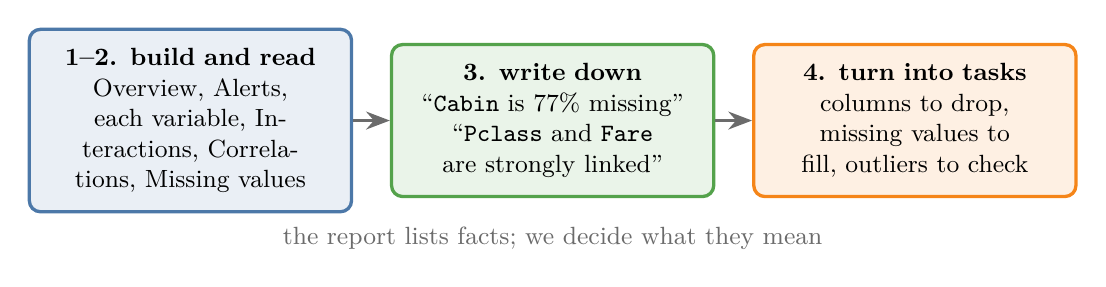
\begin{tikzpicture}[b/.style={box=#1, text width=3.6cm, minimum height=1.6cm, align=center, font=\sffamily\small}]
  \node[b=cblue] (r) at (0, 0) {\textbf{1--2. build and read}\\Overview, Alerts, each variable, Interactions, Correlations, Missing values};
  \node[b=cgreen] (o) at (4.6, 0) {\textbf{3. write down}\\``\texttt{Cabin} is 77\% missing''\\``\texttt{Pclass} and \texttt{Fare} are strongly linked''};
  \node[b=corange] (t) at (9.2, 0) {\textbf{4. turn into tasks}\\columns to drop, missing values to fill, outliers to check};
  \draw[arrow] (r) -- (o); \draw[arrow] (o) -- (t);
  \node[note] at (4.6, -1.5) {the report lists facts; we decide what they mean};
\end{tikzpicture}
\end{document}
